\section{Verwendete Geräte und Materialien}
Im Versuch werden folgende Geräte verwendet:
\begin{itemize}
    \item \textbf{Keysight FieldFox Network Analyzer N9918A}: Zur Messung der S-Parameter der Sendeplatine.
    \item \textbf{Sendeplatine}: Die Sendeplatine wird verwendet, um die Trägerfrequenz zu erzeugen und modulierte Signale zu generieren.
    \item \textbf{Empfängerplatine}: Die Empfängerplatine empfängt die modulierten Signale und demoduliert sie, um die ursprünglichen Daten wiederherzustellen. Sie wird an den FieldFox Network Analyzer N9918A angeschlossen, um die S-Parameter zu messen.
    \item \textbf{Rechner mit der Anwendung "HTerm (HyperTerminal)"}: Zur Steuerung der Sendeplatine und ggf. zum Empfang der Daten von der Empfängerplatine.
\end{itemize}
\clearpage
\section{Versuchsaufbau}
Die Abbildung~\ref{fig:Versuchsanordnung} zeigt die Versuchsanordnung und deren Verbindungen. Die Sendeplatine ist mit dem FieldFox Network Analyzer verbunden, um die S-Parameter zu messen.
\begin{figure}[H]
    \centering
    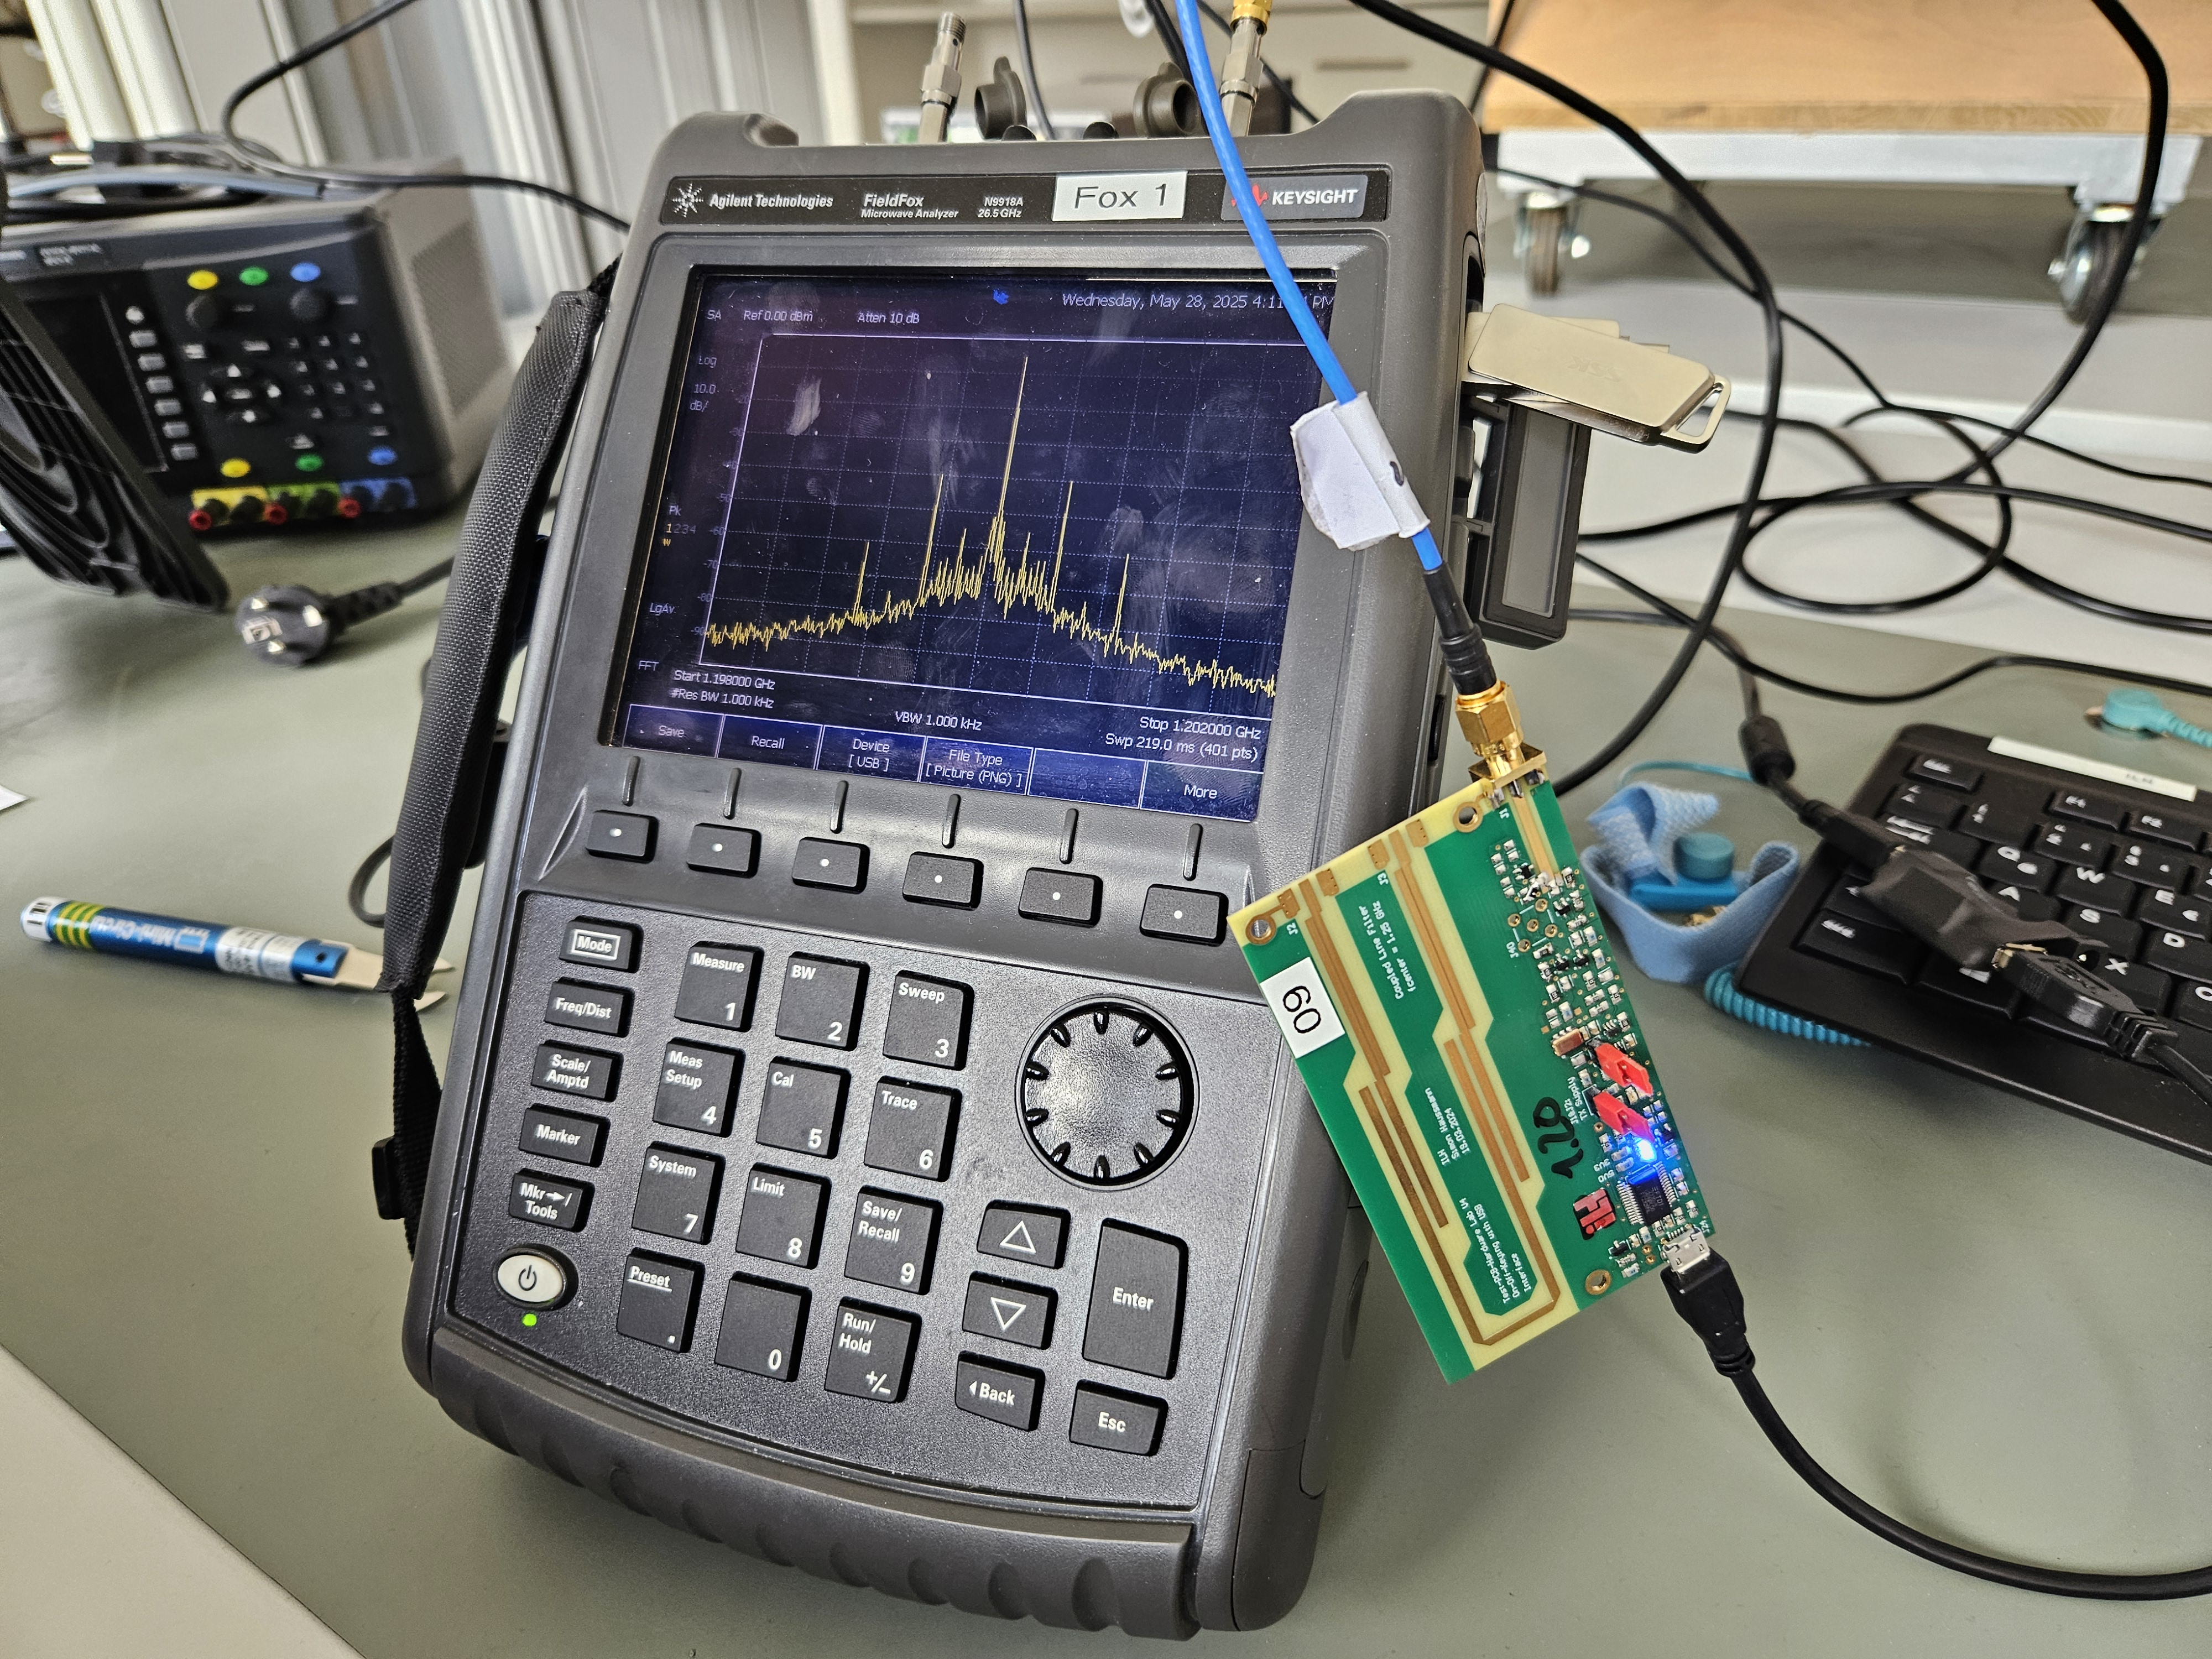
\includegraphics[width=0.8\textwidth]{Pictures/Versuchsanordnung.jpg}
    \caption{Versuchsanordnung}
    \label{fig:Versuchsanordnung}
\end{figure}
\clearpage